\section{Results}
\label{sec:results}

\subsection{Does the dataset affect quantization robustness?}

If the datasets differed only in noise, the \term{retention gap} between the two groups would scatter around zero across the grid.
Instead, bit width and group size set the overall level of retention, and the gap concentrates where retention is between its two limits (\cref{fig:curves,fig:gap}).
Averaged over the nine settings, retention is at most \V{ret_w1_max} at 1 bit and at least \V{ret_w8_min} at 8 bits for every group size.
At W3/G128, mean retention is \V{ret_w3g128}, and the UFG group retains \V{retSc_w3g128} against \V{retOther_w3g128} for the FG group, a gap of \V{gap_w3g128}.
The gap is positive in \V{gapPos_w3} of the \V{nSettingGs} combinations of setting and group size at 3 bits, and in \V{gapPos_w4} of \V{nSettingGs} at 4 bits.
Smaller groups move the transition band to fewer bits.
At W2/G8 the gap is \V{gap_w2g8}, while at W2/G128 mean retention has fallen to \V{ret_w2g128} and the gap is only \V{gap_w2g128}.
\textbf{The dataset effect is therefore a property of the transition band, and its location depends on bit width and group size together.}

\begin{figure}[t]
  \centering
  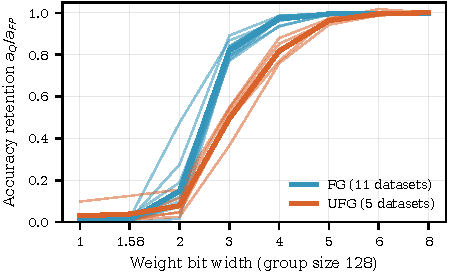
\includegraphics[width=\linewidth]{figures/retention_curves.pdf}
  \caption{Accuracy retention against weight bit width at group size 128, averaged over the nine settings. Thin lines are datasets, thick lines group means.}
  \label{fig:curves}
\end{figure}

At 1 bit, the gap is negative for BEiTv2 FT at every group size, also with the chance-corrected retention defined below.
Several UFG baselines of that backbone are close to chance, where both measures are unstable.
In \V{lowBaseline} contexts, all in the UFG group, the baseline top-1 is below 15\%.

Three checks ask whether the gap is an artifact of the retention ratio, of one benchmark or of noise (\cref{tab:robust}).
With chance-corrected retention the mean gap at W3/G128 is \V{gapChance_w3g128}, and with the baselines below 15\% removed it is \V{gapNoLow_w3g128}.
Removing any one UFG dataset leaves a gap of at least \V{looMinGap}, and cotton alone, with no soybean dataset, still retains less in every setting.
The gap is positive in all nine settings under every alternative.
Treating baseline and quantized accuracy as independent, which overstates the noise, the binomial standard error of a context's retention is at most \V{seMax} for Cotton, with 240 test images, and at most \V{seOtherMax} for any FG dataset.
A bootstrap over datasets places the 95\% interval of the gap above zero in \V{bootPositive} of the eight settings other than BEiTv2 FT, whose lower bound is \V{bootLowBeitFt}.

\begin{table}[t]
\centering
\caption{Retention gap (FG $-$ UFG) at W3/G128 under alternative definitions: the mean and minimum over the nine settings, and the settings with a positive gap. Chance correction uses $(a_{\mathrm{Q}}-1/C)/(a_{\mathrm{FP}}-1/C)$. The worst leave-one-out row removes the dataset that lowers the mean gap most.}
\label{tab:robust}
\setlength{\tabcolsep}{3pt}
\small
\begin{tabular}{lrrr}
\toprule
Check & Mean & Min & Positive (of 9) \\
\midrule
Main analysis & 0.33 & 0.17 & 9 \\
Chance-corrected retention & 0.34 & 0.18 & 9 \\
Baselines below 15\% removed & 0.36 & 0.17 & 9 \\
Soybean datasets as one unit & 0.31 & 0.17 & 9 \\
Cotton alone & 0.27 & 0.08 & 9 \\
Soybean datasets alone & 0.34 & 0.18 & 9 \\
Leave out one dataset (worst) & 0.29 & 0.15 & 9 \\
\bottomrule
\end{tabular}
\end{table}


\begin{figure*}[t]
  \centering
  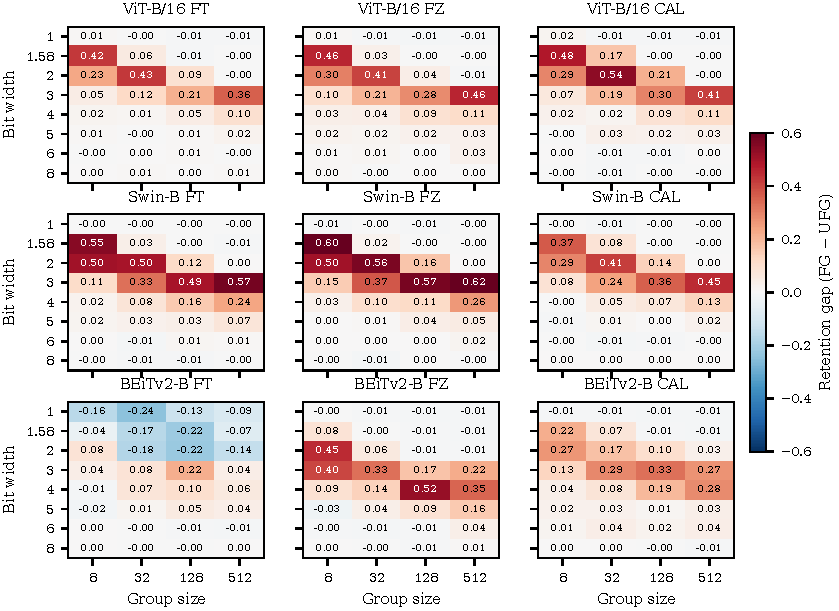
\includegraphics[width=\linewidth]{figures/gap_heatmaps.pdf}
  \caption{Retention gap (FG $-$ UFG) for each backbone and fine-tuning strategy, by bit width and group size. Positive values mean the UFG datasets retain less. Group means weight the datasets equally.}
  \label{fig:gap}
\end{figure*}

If the dataset drives the difficulty, the datasets should also keep their order when the quantization condition, the backbone or the strategy changes.
Within each setting, the four primary conditions agree well, with Kendall's $W$ between \V{wMin} and \V{wMax} (\cref{tab:gates}).
The \term{difficulty score} is therefore a common ranking within each setting.
Across settings the agreement is weaker (\cref{fig:agreement}).
The median Spearman correlation between the scores of two settings is \V{agreeMedian}, and it ranges from \V{agreeMin} to \V{agreeMax}.
BEiTv2 CAL and BEiTv2 FT agree least, so the backbone alone does not fix the ranking.
However, a rank correlation counts every exchange of two datasets equally, also between FG datasets whose retention is close.
Among the FG datasets alone, the median correlation between two settings is only \V{agreeOtherMedian}.
The order between the groups is more stable.
In each setting, we take every pair of one UFG and one FG dataset and count the share in which the UFG dataset has the higher score.
This share is at least \V{sepMin}, and it is one in \V{sepOne} of nine settings.
The UFG datasets hold at least \V{scHardestMin} of the five hardest places in every setting, and all five in \V{scHardestAll} settings.
\textbf{The dataset effect is stable at the level of the two groups, while the order within the FG group depends on the backbone and the strategy.}

\begin{figure}[t]
  \centering
  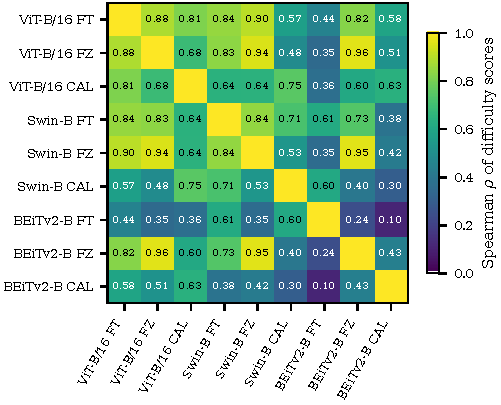
\includegraphics[width=\linewidth]{figures/ranking_agreement.pdf}
  \caption{Spearman correlation between the difficulty scores of the \V{gridDatasets} datasets in each pair of settings.}
  \label{fig:agreement}
\end{figure}

\subsection{How and why does the dataset affect quantization robustness?}

\paragraph{Logit margin.}
If quantization perturbs logits by a similar amount everywhere, images with small baseline margins should change first, and datasets with many such images should lose more.
The prespecified margin signal holds in all \V{gatePass} settings (\cref{tab:gates}).
The median correlation between $q_{10}$ and the \term{difficulty score} is \V{rhoMarginMedian}, and the permutation test gives $p<0.05$ in all \V{gatePPass} settings.
However, baseline accuracy correlates with the score almost as strongly, with a median $\rho$ of \V{rhoAccMedian}.
Adding $q_{10}$ to baseline accuracy and the log number of classes lowers the held-out error in only \V{marginHelps} of nine settings.
A rank correlation that controls for baseline accuracy separates the two predictors.
The partial correlation between $q_{10}$ and the score is negative in \V{partialNeg} of nine settings, with a median of \V{partialMedian}.
\textbf{The margin adds rank information beyond baseline accuracy, but not enough to improve a held-out linear prediction.}

\begin{table}[t]
\centering
\caption{Difficulty score of the {\V{gridDatasets}} datasets. $W$: agreement of the four primary conditions. $\rho$: Spearman correlation of the score with the baseline margin $q_{10}$ (one-sided permutation $p$) and with FP top-1. Err: leave-one-dataset-out squared error ($\times 10^{3}$) of the controls (Ctrl.) alone and with $q_{10}$ added.}
\label{tab:gates}
\setlength{\tabcolsep}{1.8pt}
\small
\begin{tabular}{llrrrrrr}
\toprule
 & & & \multicolumn{2}{c}{Margin $q_{10}$} & FP top-1 & \multicolumn{2}{c}{Err $\downarrow$} \\
\cmidrule(lr){4-5}\cmidrule(lr){7-8}
Backbone & Strategy & $W$ $\uparrow$ & $\rho$ & $p$ & $\rho$ & Ctrl. & +$q_{10}$ \\
\midrule
ViT-B/16 & FT & 0.89 & $-$0.96 & $<$0.01 & $-$0.97 & 17.7 & 36.5 \\
ViT-B/16 & FZ & 0.93 & $-$0.93 & $<$0.01 & $-$0.91 & 17.1 & 140.4 \\
ViT-B/16 & CAL & 0.81 & $-$0.82 & $<$0.01 & $-$0.84 & 20.9 & 19.8 \\
Swin-B & FT & 0.81 & $-$0.87 & $<$0.01 & $-$0.82 & 36.9 & 51.8 \\
Swin-B & FZ & 0.95 & $-$0.97 & $<$0.01 & $-$0.98 & 12.3 & 110.7 \\
Swin-B & CAL & 0.73 & $-$0.65 & $<$0.01 & $-$0.67 & 54.5 & 63.1 \\
BEiTv2-B & FT & 0.83 & $-$0.53 & 0.02 & $-$0.45 & 117.5 & 83.9 \\
BEiTv2-B & FZ & 0.94 & $-$0.93 & $<$0.01 & $-$0.96 & 12.3 & 59.6 \\
BEiTv2-B & CAL & 0.91 & $-$0.80 & $<$0.01 & $-$0.72 & 53.8 & 36.2 \\
\bottomrule
\end{tabular}
\end{table}


Baseline accuracy also leaves the retention of individual contexts open (\cref{fig:accuracy}).
Over the \V{pooledN} contexts at W3/G128, it explains \V{pooledR2}\% of the variance of retention in a linear fit.
Within one setting, \V{pairsClose} pairs of datasets have baseline top-1 within 1.5 points of each other, and \V{pairsDiffer} of them differ in retention by more than 0.2, by up to \V{pairsMaxDiff}.
In \V{pairsQ10} of the \V{pairsClose} pairs, and in \V{differQ10} of the \V{pairsDiffer}, the dataset with the smaller $q_{10}$ retains less.
On BEiTv2 CAL, Cars and Food start from \V{pairALowFp}\% and \V{pairAHighFp}\% but retain \V{pairALowR} and \V{pairAHighR}, and Cars has the smaller $q_{10}$, \V{pairALowQ} against \V{pairAHighQ}.
On BEiTv2 FT, Dogs and Cars start from \V{pairBLowFp}\% and \V{pairBHighFp}\% and retain \V{pairBLowR} and \V{pairBHighR}, but here Dogs has the larger $q_{10}$, \V{pairBLowQ} against \V{pairBHighQ}.
On Swin-B CAL, SoyGene and iNat17 start from \V{pairCLowFp}\% and \V{pairCHighFp}\%, and the soybean dataset retains \V{pairCLowR} against \V{pairCHighR}.
In each pair the same dataset retains less in all four primary conditions, so the differences are not specific to W3/G128.

\begin{figure}[t]
  \centering
  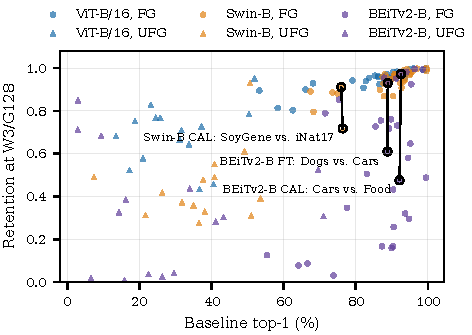
\includegraphics[width=\linewidth]{figures/accuracy_retention.pdf}
  \caption{Retention at W3/G128 against baseline top-1 for the \V{pooledN} contexts. Lines join three pairs from one setting with nearly equal baseline accuracy.}
  \label{fig:accuracy}
\end{figure}

Margin matching asks how much of the gap between the groups goes with their margins, within the W3/G128 test images.
The UFG images concentrate at small margins, while the FG images spread over a long tail (\cref{fig:margin}).
Matching both groups to their common margin distribution reduces the \term{retention gap} by \V{reductionMin}\% to \V{reductionMax}\% across the nine settings, with a median of \V{reductionMedian}\% (\cref{tab:margin}).
The matched gap stays positive in \V{matchedPositive} of nine settings, so the UFG images lose more even at equal margin.
The comparison covers only the shared part of the distributions, an overlap of \V{overlapMin} to \V{overlapMax} of the histogram mass.
The matched ESS falls to as little as \V{essRatioMin}\% of the raw ESS, and the largest image weight is \V{weightMax} times its raw weight.

\begin{figure}[t]
  \centering
  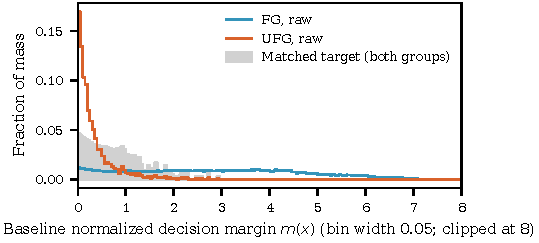
\includegraphics[width=\linewidth]{figures/margin_distribution.pdf}
  \caption{Baseline margin distributions of the two groups for ViT-B/16 FT, before matching, and the common target used for matching. Margins above 8 are not shown.}
  \label{fig:margin}
\end{figure}

\begin{table}[t]
\centering
\caption{Retention gap (FG $-$ UFG) at W3/G128 before and after matching the baseline margin distributions, bin width 0.05. Red.: reduction of the gap. Overlap is the shared histogram mass; ESS is the lower of the two groups' matched-to-raw effective sample size.}
\label{tab:margin}
\setlength{\tabcolsep}{1.6pt}
\small
\begin{tabular}{llrrrrr}
\toprule
Backbone & Strategy & Raw & Matched & Red. (\%) & Overlap & ESS (\%) \\
\midrule
ViT-B/16 & FT & 0.212 & 0.042 & 80.0 & 0.26 & 23.4 \\
ViT-B/16 & FZ & 0.310 & 0.188 & 39.2 & 0.40 & 42.6 \\
ViT-B/16 & CAL & 0.268 & 0.118 & 55.9 & 0.24 & 29.6 \\
Swin-B & FT & 0.498 & 0.248 & 50.2 & 0.23 & 26.3 \\
Swin-B & FZ & 0.569 & 0.412 & 27.6 & 0.34 & 32.9 \\
Swin-B & CAL & 0.341 & 0.112 & 67.1 & 0.26 & 31.9 \\
BEiTv2-B & FT & 0.408 & 0.188 & 53.9 & 0.19 & 20.9 \\
BEiTv2-B & FZ & 0.184 & 0.078 & 57.4 & 0.37 & 34.1 \\
BEiTv2-B & CAL & 0.325 & 0.061 & 81.3 & 0.34 & 47.5 \\
\bottomrule
\end{tabular}
\end{table}


\begin{figure*}[t]
  \centering
  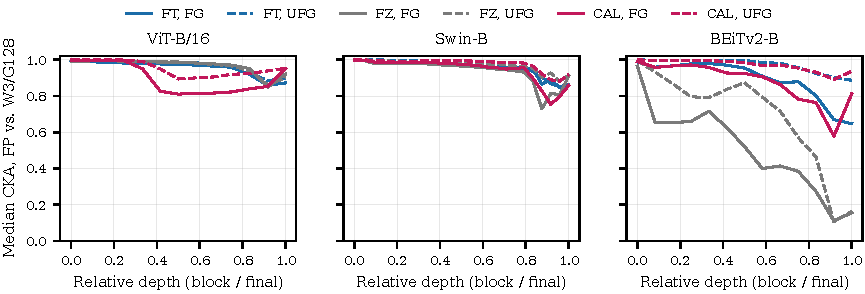
\includegraphics[width=\linewidth]{figures/layer_cka.pdf}
  \caption{Median linear CKA between baseline and W3/G128 features after each block, over the datasets of each group. Depth is the block index divided by the number of positions; Swin-B has 25 positions, the others 13.}
  \label{fig:cka}
\end{figure*}

Matching aligns only the distance to the second-ranked class, but most swaps do not go to that class.
Over the \V{beyondContexts} contexts at W3/G128, a median of \V{beyondMedian}\% of swaps end on a class the baseline ranked below second; rank-2 and rank-3 ties count as second.
This share is \V{beyondSc}\% for the UFG contexts and \V{beyondOther}\% for the FG contexts, and every UFG dataset has a higher share than every FG dataset.
It does not follow the number of classes: Cotton with \V{cottonClasses} classes reaches \V{beyondCotton}\%, against \V{beyondCub}\% for CUB with \V{cubClasses}, and the correlation with the class count is \V{beyondRhoClasses}.
It follows the margin instead, with a correlation of \V{beyondRhoMargin} with $q_{10}$.
The top-1 to top-2 margin is therefore a summary of how close the baseline decisions are, not a full account of how quantization changes them, which is consistent with the positive matched gap.
\textbf{Much of the retention gap goes with the smaller margins of the UFG images, but the margin does not account for all of it.}
Margins to lower-ranked classes, of which the competitor counts below are a first form, are the next diagnostic.

\paragraph{Feature changes.}
If quantization damaged the features of the hard datasets more, their quantized features should drift further from the baseline.
\Cref{fig:cka} shows the opposite in the middle of the network.
Over all contexts at relative depths between 0.45 and 0.55, the median CKA between baseline and W3/G128 features is \V{midCkaSc} for the UFG group and \V{midCkaOther} for the FG group.
The final-layer CKA correlates only weakly with the \term{difficulty score}, with a median $\rho$ of \V{rhoCkaMedian} (\cref{tab:properties}).
Among baseline properties, separability tracks the score with a median $\rho$ of \V{rhoSepMedian}, as baseline accuracy does, while the H-score and the norm ratio P99/P50 do not, at \V{rhoHscoreMedian} and \V{rhoNormMedian}.
The one setting where features collapse is BEiTv2 LP.
Its median final CKA is \V{beitFzCka} (\cref{tab:diagnostics}), and its mean accuracy falls from \V{beitFzFp}\% to \V{beitFzQ}\% (\cref{tab:w3}).
\textbf{Feature similarity identifies a collapsed backbone, but it does not rank the datasets by accuracy loss.}

\begin{table}[t]
\centering
\caption{W3/G128 results over the {\V{nDatasets}} datasets. FP and Q: baseline and quantized top-1. Accuracies, swap, damage and rescue rates are dataset means in \%; the relative loss is the dataset median.}
\label{tab:w3}
\setlength{\tabcolsep}{2.2pt}
\small
\begin{tabular}{llrrrrrr}
\toprule
Backbone & Strategy & FP & Q & Loss $\downarrow$ & Swap & Damage & Rescue \\
\midrule
ViT-B/16 & FT & 70.7 & 65.5 & 6.1 & 25.8 & 8.1 & 2.9 \\
ViT-B/16 & FZ & 62.8 & 56.1 & 8.5 & 35.0 & 9.9 & 3.2 \\
ViT-B/16 & CAL & 72.0 & 67.3 & 3.5 & 25.5 & 7.4 & 2.7 \\
Swin-B & FT & 72.5 & 62.6 & 9.3 & 32.8 & 12.1 & 2.2 \\
Swin-B & FZ & 69.6 & 59.5 & 10.6 & 34.8 & 12.7 & 2.6 \\
Swin-B & CAL & 79.3 & 70.7 & 5.1 & 23.6 & 10.6 & 2.1 \\
BEiTv2-B & FT & 65.0 & 50.4 & 25.7 & 38.4 & 16.3 & 1.7 \\
BEiTv2-B & FZ & 62.9 & 12.3 & 89.4 & 87.5 & 51.2 & 0.6 \\
BEiTv2-B & CAL & 76.4 & 50.1 & 44.8 & 46.6 & 28.0 & 1.8 \\
\bottomrule
\end{tabular}
\end{table}


\paragraph{Decision changes.}
Accuracy loss is the difference between damage and rescue.
Damage exceeds rescue in every setting, by a factor of at least \V{damageOverRescueMin} (\cref{tab:w3}).
The UFG group has the higher mean swap rate in \V{swapHigherSc} of nine settings.

Class-dependent logit offsets explain part of the damage (\cref{tab:diagnostics}).
The cross-fitted offset correction raises mean top-1 by \V{biasGainMin} to \V{biasGainMax} points, while the shuffled controls lower it in every setting, by \V{shuffleLossMin} to \V{shuffleLossMax} points.
The gain is therefore specific to the class of the offset.
Competing classes add little beyond the margin.
Adding the competitor counts lowers the damage Brier score in \V{competitorBetter} of nine settings, but raises it for ViT-B/16 FT and BEiTv2 FT.
AUROC is undefined in \V{aurocUndefined} of \V{aurocRows} evaluations, where every held-out baseline-correct image is damaged; we report these as missing.

\subsection{Limitations}

Each dataset is tied to the checkpoints trained on it, so the dataset differences are associations, not effects of the data alone.
The two groups differ in domain, class count, training-set size and baseline accuracy at once, and this study cannot separate these factors.
Each context has one checkpoint and one inference seed, so we report no uncertainty across training runs.
The paired feature and logit analyses cover W3/G128 only.
Margin matching compares the groups only on their shared margin range, and the offset correction is fitted on test logits.
